\documentclass[runningheads]{LaTeX2e_Proceedings_Templates/llncs}

\usepackage{graphicx}
\usepackage{booktabs}
\usepackage{amssymb}
\usepackage[table]{xcolor}

\definecolor{rankbest}{HTML}{F4B7B7}
\definecolor{ranksecond}{HTML}{F7D7A1}
\definecolor{rankthird}{HTML}{FFF1A8}
\newcommand{\best}[1]{\cellcolor{rankbest}\textbf{#1}}
\newcommand{\second}[1]{\cellcolor{ranksecond}\textbf{#1}}
\newcommand{\third}[1]{\cellcolor{rankthird}\textbf{#1}}
\newcommand{\cmark}{\checkmark}
\newcommand{\xmark}{--}

\begin{document}

\title{UAV-TAlign: Scene-Level RGB-Thermal Alignment for Cross-FOV UAV Imagery}
\titlerunning{UAV-TAlign}

\author{Anonymous Authors}
\authorrunning{Anonymous Authors}

\institute{Anonymous submission for PRCV 2026}

\maketitle

\begin{abstract}
UAV RGB-thermal alignment is a core capability for inspection, monitoring, and nighttime
multimodal perception, yet real aerial data expose a gap between strong pairwise matching and
reliable scene-level alignment. Viewpoint variation, cross-resolution sensing, thermal rendering
changes, and low-light imagery make individual homographies uneven even when modern multimodal
matchers return abundant correspondences. We present UAV-TAlign, a scene-level RGB-thermal
alignment framework that turns state-of-the-art pairwise multimodal matching into robust
scene-level alignment through reliability-guided evidence selection, robust homography consensus,
and QA-aware scene verification. We also package UAV-TAlign-1K with a practical label-free
evaluation protocol for real UAV RGB-thermal alignment. Experiments against classical and modern
off-the-shelf baselines, protocol-consistency analysis, and cumulative module ablations show that
the decisive gains come from robust scene consensus and reliability-aware verification, rather than
from pairwise matcher availability alone.

\keywords{RGB-thermal registration \and UAV imagery \and multimodal alignment \and scene-level
reliability}
\end{abstract}

% !TEX root = ../paper.tex

\section{Introduction}

RGB-thermal alignment is a core capability for UAV inspection, monitoring, and low-light
perception, where visible and thermal imagery provide complementary scene cues across
multispectral pedestrian analysis, thermal object detection, visible-thermal tracking, and UAV
multimodal perception
\cite{hwang2015kaist,flir2018thermal,jia2021llvip,liu2022tardal,sun2022dronevehicle,zhang2022vtuav,li2022lasher,jiang2023antiuav}.
In real deployments, however, reliable registration is difficult because UAV RGB-thermal data often
combine viewpoint change, cross-resolution sensors, weak thermal texture, grayscale or pseudocolor
thermal rendering, and day/night illumination variation. These factors make scene-level alignment
substantially harder than standard same-view or near-same-view multimodal matching setups.

Recent multimodal matchers have significantly improved pairwise cross-modal correspondence
estimation, and strong off-the-shelf models can already produce usable registrations for many
individual RGB-thermal pairs
\cite{sarlin2020superglue,sun2021loftr,chen2022aspanformer,lindenberger2023lightglue,edstedt2023dkm,edstedt2024roma,tuzcuoglu2024xoftr,ren2025minima}.
Yet our experiments show that high pairwise usability does not automatically translate into
reliable scene-level alignment under realistic UAV conditions. This exposes a system-level gap:
state-of-the-art pairwise matchers can make correspondences available, but UAV RGB-thermal
alignment still requires a mechanism that consolidates evidence across a scene and verifies whether
the resulting transform is reliable enough to use.

This observation motivates a shift in problem framing. Rather than treating UAV RGB-thermal
registration primarily as a pairwise matching availability problem, we study it as a scene-level
reliability problem. Under this view, the central question becomes how to convert strong but
imperfect pairwise registrations into scene-level transforms that remain geometrically stable,
internally consistent, and usable after QA-aware acceptance.

To address this problem, we present UAV-TAlign, a scene-level UAV RGB-thermal alignment framework
that complements modern multimodal matchers rather than competing with them as another local
matcher. UAV-TAlign combines reliability-guided evidence selection, robust homography consensus,
and QA-aware scene verification to convert strong pairwise correspondences into scene-level
alignment decisions. We further package UAV-TAlign-1K, a public subset and practical label-free
evaluation setup for studying real UAV RGB-thermal alignment without requiring manual landmark
annotation as a prerequisite.

Our contributions are threefold:
\begin{itemize}
\item We present UAV-TAlign, a scene-level UAV RGB-thermal alignment framework that elevates
state-of-the-art pairwise multimodal matching into reliable scene-level alignment through
reliability-guided evidence selection, robust homography consensus, and QA-aware verification.
\item We package UAV-TAlign-1K as a public evaluation subset together with a practical label-free
evaluation protocol for real UAV RGB-thermal alignment, without requiring manual landmark
annotations as a prerequisite.
\item Extensive baseline comparisons, protocol-consistency analysis, and cumulative module
ablations show that the dominant empirical gains come from scene-level reliability modeling rather
than pairwise matcher availability alone.
\end{itemize}

% !TEX root = ../paper.tex

\section{Related Work}

\subsection{Classical Image Registration}

Classical image registration pipelines typically rely on hand-crafted local features followed by
robust geometric fitting. Representative methods built on SIFT, SURF, ORB, BRISK, KAZE, or AKAZE
remain attractive because they are simple, interpretable, and do not require task-specific
training
\cite{lowe2004sift,bay2008surf,rublee2011orb,leutenegger2011brisk,alcantarilla2012kaze,alcantarilla2013akaze}.
However, their performance can degrade substantially in cross-modal settings, especially when the
appearance gap between visible and thermal imagery reduces descriptor repeatability or when thermal
frames contain weak texture and large homogeneous regions.

These methods remain important baselines in our study because they represent the classical
registration view of the problem: if sufficiently stable local features can be extracted, a single
pairwise homography may already solve the task. Robust model estimation remains central in these
pipelines, from RANSAC and multiple-view geometry to more recent variants such as MAGSAC and
MAGSAC++
\cite{fischler1981ransac,hartley2004multiple,barath2019magsac,barath2020magsacpp}. Our results
suggest that the single-pair assumption is too weak for real UAV RGB-thermal scenes, where
scene-level reliability often remains difficult even when some individual pairs are usable.

\subsection{Deep Pairwise Matching for Multimodal Registration}

Recent dense and semi-dense matching methods have significantly improved pairwise geometric
correspondence estimation. Learned local features have evolved from trainable detectors and
descriptors such as SuperPoint, LF-Net, D2-Net, R2D2, DISK, S2DNet, HardNet, L2-Net, SOSNet,
GeoDesc, ContextDesc, ASLFeat, ALIKE, and Key.Net
\cite{detone2018superpoint,ono2018lfnet,dusmanu2019d2net,revaud2019r2d2,tyszkiewicz2020disk,germain2020s2dnet,mishchuk2017hardnet,tian2017l2net,tian2019sosnet,luo2018geodesc,luo2019contextdesc,luo2020aslfeat,zhao2023alike,barroso2019keynet},
while match filtering and end-to-end correspondence reasoning have progressed through
SuperGlue, NCNet, Patch2Pix, COTR, LoFTR, ASpanFormer, LightGlue, DKM, RoMa, Efficient LoFTR,
OmniGlue, MINIMA, and XoFTR
\cite{sarlin2020superglue,rocco2018ncnet,zhou2021patch2pix,jiang2021cotr,sun2021loftr,chen2022aspanformer,lindenberger2023lightglue,edstedt2023dkm,edstedt2024roma,wang2024efficientloftr,jiang2024omniglue,ren2025minima,tuzcuoglu2024xoftr}.
In particular, these methods are better at recovering useful correspondences in weak-texture
regions, repetitive structures, or substantial appearance shifts. Broad reviews of this transition
from classical pipelines to trainable matching, together with practical benchmarking studies,
provide additional context
\cite{ma2021survey,liao2024survey}.

Our work builds directly on this progress instead of trying to replace it. The empirical picture in
UAV-TAlign-1K is that strong off-the-shelf multimodal matchers already provide very high pairwise
availability. This changes the central question. The bottleneck is no longer only whether a matcher
can produce correspondences for a given RGB-thermal pair, but whether those frame-level estimates
can be converted into a stable and reliable scene-level alignment under realistic UAV operating
conditions.

\subsection{Visible-Thermal Registration and Evaluation}

Visible-thermal registration has been studied under a range of assumptions, from same-view or
near-same-view alignment to broader multimodal correspondence learning. Radiation-variation
insensitive matching methods such as RIFT and deep alignment or stitching formulations such as
CLKN and UDIS indicate the breadth of existing registration formulations
\cite{li2020rift,chang2017clkn,nie2021udis}. Many existing settings either operate under relatively
controlled viewpoint changes or evaluate pairwise registration in a way that does not require a
scene-level acceptance decision. By contrast, practical UAV RGB-thermal data frequently combine
cross-FOV capture, cross-resolution sensing, thermal rendering variation, and low-light conditions.
These factors make scene-level reliability a more central concern than in many standard
visible-thermal evaluation setups.

A further complication is that point-level manual geometric ground truth is expensive and sometimes
ill-posed in weak-texture thermal frames. For the current PRCV scope, we therefore avoid presenting
our dataset package as a fully supervised benchmark. Instead, we package a public subset,
UAV-TAlign-1K, together with a practical label-free evaluation protocol that measures
scene-consistency and relative alignment quality without requiring manual landmark annotation as a
prerequisite.

\subsection{UAV Multimodal Datasets and the Remaining Gap}

UAV multimodal datasets have supported progress in detection, tracking, segmentation, and broader
cross-modal perception, spanning aligned pedestrian and automotive benchmarks as well as
RGB-thermal detection and tracking benchmarks such as KAIST, FLIR, LLVIP, M3FD, DroneVehicle,
VTUAV, LasHeR, and Anti-UAV
\cite{hwang2015kaist,flir2018thermal,jia2021llvip,liu2022tardal,sun2022dronevehicle,zhang2022vtuav,li2022lasher,jiang2023antiuav}.
However, registration is not always the primary task in those benchmarks, and the protocol
assumptions needed for scene-level RGB-thermal alignment are often different from those needed for
downstream semantic tasks. In particular, a practical registration pipeline must decide not only
how to align frames, but also when the scene-level evidence is strong enough to trust the
resulting transform.

This is the gap our paper targets. Rather than introducing a new matcher architecture, we focus on
a practical scene-level registration setting for real UAV RGB-thermal imagery. Our contribution
lies in the combination of a reliability-oriented pipeline, a public subset packaging, and a
label-free protocol that makes the problem studyable without first building dense manual geometric
annotations.

% !TEX root = ../paper.tex

\section{UAV-TAlign-1K and Evaluation Protocol}

\subsection{Dataset Scope}

We package UAV-TAlign-1K as a focused public evaluation subset for real UAV RGB-thermal
registration. The subset contains 15 scenes, 500 RGB-thermal pairs, and 1000 images in total. Each
sample is organized as an RGB image paired with a thermal image captured from the same scene
context, while the dataset as a whole spans practical UAV conditions that go beyond standard
near-same-view multimodal matching. In scope and modality, it is closer to recent RGB-thermal
benchmarks such as
KAIST, FLIR, LLVIP, M3FD, DroneVehicle, VTUAV, LasHeR, and Anti-UAV than to classical
same-sensor image matching setups
\cite{hwang2015kaist,flir2018thermal,jia2021llvip,liu2022tardal,sun2022dronevehicle,zhang2022vtuav,li2022lasher,jiang2023antiuav}.

At the scene level, the subset preserves the factors that make reliability assessment meaningful:
day, night, and low-light capture; grayscale and pseudocolor thermal rendering; and both wide-view
and zoom-view scene families. The packaged formal split includes 7 day scenes, 5 night scenes, and
3 low-light scenes; 8 grayscale-thermal scenes and 7 pseudocolor-thermal scenes; and paired
wide/zoom controls for the substation scene family.

\begin{figure}[t]
\centering
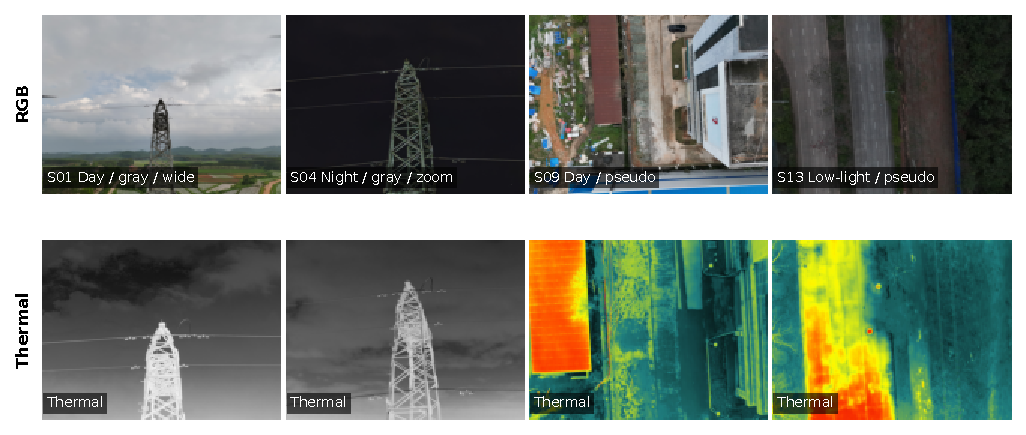
\includegraphics[width=\textwidth]{figures/fig_dataset_examples.pdf}
\caption{Representative UAV-TAlign-1K RGB-thermal pairs spanning day, night, low-light,
grayscale-thermal, pseudocolor-thermal, wide-view, and zoom-view conditions.}
\label{fig:dataset_examples}
\end{figure}

\subsection{Dataset Organization}

Each scene is stored under its own scene directory, and paired samples are formed by matching file
stems between \texttt{rgb/} and \texttt{thermal/} subdirectories. The dataset loader constructs
scene pairs from common RGB and thermal filenames, while scene-level metadata are loaded from the
subset manifest. For each pair, the loader stores scene identity, pair identity, light condition,
thermal rendering, view type, and scene label.

This organization supports both pairwise baseline evaluation and scene-level pipeline evaluation
under the same subset definition, while also enabling condition-based breakdowns from a unified
scene manifest.

\subsection{Complementary Evaluation Units}

The protocol uses two complementary evaluation units. First, off-the-shelf baselines are evaluated
at the pair level. Each of the 500 RGB-thermal pairs is processed independently, and the resulting
statistics describe whether a method can produce a usable pairwise registration and homography
under a fixed off-the-shelf setting.

Second, UAV-TAlign is evaluated at the scene level. Multiple frame-level estimates are aggregated
into a scene-level transform, and the final decision is made by canonical scene acceptance rather
than by pairwise usability alone. The pairwise and scene-level tables therefore provide two
complementary views of practical registration behavior: correspondence availability and retained
scene-level alignment reliability.

\subsection{Label-Free QA Proxies}

The protocol relies on label-free relative QA signals designed for scalable scene-level reliability
analysis. The strongest stored proxies compare the optimized transform against a baseline
initialization and summarize whether scene-level rectification improves cross-modal agreement. The
proxy family includes edge-overlap improvement, gradient-NCC improvement, the ratio of
frames with improved gradient agreement, severe baseline-relative outlier count and ratio,
accepted-frame ratio, and homography-dispersion and robust-rejection diagnostics.

These proxies provide a practical scene-consistency signal for comparing methods and for deciding
whether a scene-level transform is reliable enough to retain, in the spirit of practical
matching-oriented evaluation and benchmarking discussed in prior image-matching literature
\cite{ma2021survey,liao2024survey}.

% !TEX root = ../paper.tex

\section{Method}

\subsection{Problem Formulation}

We study RGB-thermal registration as a scene-level alignment task. For each scene, the input is a
set of paired RGB and thermal UAV frames
$S = \{(I_i^R, I_i^T)\}_{i=1}^N$, where viewpoint variation, cross-resolution sensing, thermal
appearance changes, and day/night conditions make individual frame estimates uneven in quality. The
goal is to recover a thermal-to-RGB homography that remains reliable at the scene level, with the
canonical output retained when the evidence satisfies the reliability criterion.

This formulation turns registration from a single best-pair problem into a multi-frame reliability
optimization problem. In our setting, many scenes already contain usable pairwise correspondences,
but the central challenge is to convert uneven frame-level estimates into a transform that is
geometrically stable, internally consistent, and acceptable under a reliability-aware criterion.

\begin{figure}[t]
\centering
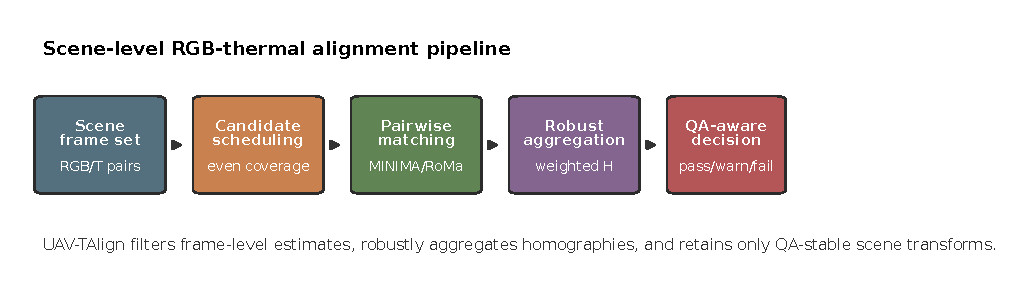
\includegraphics[width=\textwidth]{figures/fig_method_pipeline.pdf}
\caption{Overview of UAV-TAlign. The framework builds on strong pairwise matching, but
makes the final decision at the scene level through reliability-guided evidence selection, robust
homography consensus, and QA-aware verification.}
\label{fig:method_pipeline}
\end{figure}

\subsection{Pairwise Evidence Backbone}

UAV-TAlign uses a strong off-the-shelf multimodal matcher as its pairwise evidence generator. Our
PRCV implementation uses the MINIMA family with the RoMa branch as the default backend, while the
rest of the pipeline remains agnostic to the exact pairwise matcher
\cite{edstedt2024roma,ren2025minima}.

\subsection{Reliability-Guided Evidence Selection}

At the scene level, UAV-TAlign prioritizes the most informative frame evidence before expanding the
support set. It uses a progressive evidence schedule that expands with scene size and can cover all
frames when needed. This reliability-guided policy allows the framework to stop when a compact
subset already yields a stable consensus, while still escalating to broader evidence when the scene
benefits from more support.

Within each stage, representative frames are selected with deterministic evenly distributed
sampling by default. A random-selection variant is used only for sensitivity analysis. The default
policy is therefore framed as a reproducible operating choice that reduces seed-dependent drift and
preserves uniform scene coverage.

\subsection{Quality-Weighted Frame Geometry}

For each selected frame pair, the matcher produces cross-modal correspondences that are filtered
into a frame-level homography estimate. UAV-TAlign evaluates each frame using
standard geometric statistics, including the number of matches, the number of inliers, inlier
ratio, reprojection error, and spatial coverage. A frame enters the global candidate pool only when
it passes a geometry-quality gate on these statistics. The overall geometric treatment remains rooted
in standard homography estimation and robust fitting practice
\cite{hartley2004multiple,fischler1981ransac,barath2019magsac,barath2020magsacpp}.

Beyond a binary accept/reject decision, the pipeline assigns each accepted frame a quality score so
that better-supported homographies receive more influence during scene aggregation. The score is a
weighted combination of inlier ratio, spatial coverage, reprojection quality, matcher confidence,
and inlier count. This keeps the scene-level estimate from being dominated by low-support frames
that only marginally satisfy the frame-level gate.

\subsection{Robust Scene Consensus}

Once enough frame-level homographies have been accepted, UAV-TAlign forms a scene-level consensus.
Homographies are mapped into parameter space, centered with a median reference, and filtered by a
median-absolute-deviation rule to suppress unstable estimates before weighted averaging. The
retained homographies are then combined using the frame quality scores defined above.

The pipeline records stability diagnostics around the aggregate transform, including homography
dispersion relative to the aggregate and the ratio of robustly rejected frame-level estimates.
These diagnostics connect consensus formation with the final QA-aware decision.

\subsection{QA-Aware Scene Verification}

The final decision integrates match availability with scene-level reliability evidence. UAV-TAlign
evaluates the optimized scene-level transform against a label-free QA summary computed on
representative frames. The current summary uses cross-modal proxy signals such as edge-overlap
improvement, gradient-NCC improvement, the ratio of improved frames, and the count of severe
relative outliers. It also retains scene-level match and stability statistics such as accepted-frame
ratio, mean inlier ratio, mean reprojection error, spatial coverage, dispersion relative to the
aggregate transform, and the robust reject ratio.

The canonical decision uses a baseline-aware verification rule. A scene is retained when
accepted-frame statistics remain strong, the aggregated homography is stable, severe
baseline-relative outliers remain controlled, and the transform improves gradient-based alignment
beyond configured floors. This final verification step gives UAV-TAlign its scene-level character:
the framework optimizes for reliable alignment products rather than merely maximizing the number of
matched frames.

% !TEX root = ../paper.tex

\section{Experimental Setup}

\subsection{Baselines}

We evaluate both classical and learning-based baselines under an explicit off-the-shelf setting.
All learning-based methods use public pretrained weights or public pretrained model interfaces, and
none of the baselines are retrained or fine-tuned on UAV-TAlign-1K. This choice keeps the
comparison focused on practical deployability rather than dataset-specific adaptation.

The classical baselines are SIFT + RANSAC and AKAZE + RANSAC. The deep pairwise baselines are
Kornia LoFTR (pretrained="outdoor"), official pretrained RoMa via local wrapper, official
pretrained XoFTR-640 via local wrapper, and raw MINIMA. Raw MINIMA uses the MINIMA RoMa branch in
its direct pairwise form, without the scene-level candidate selection, robust multi-frame
aggregation, or QA-aware decision logic introduced by UAV-TAlign.

\subsection{Shared Geometric Fitting}

For the pairwise methods, the common downstream step is homography fitting from the predicted
correspondences. After each matcher returns point pairs and optional confidence values, the
evaluation script estimates a homography with a shared robust backend and then records a unified
status code such as \texttt{ok}, \texttt{fit\_failed}, \texttt{insufficient\_matches},
\texttt{no\_matches}, or \texttt{error}. This unified post-processing is important because it makes
the pairwise baseline table comparable at the level of usable registration outcomes rather than raw
matcher outputs alone.

The current homography fitting backend uses the same configuration across pairwise baselines:
\begin{itemize}
\item robust fitting method: USAC-MAGSAC;
\item reprojection threshold: 3.0;
\item confidence: 0.999;
\item maximum iterations: 10000;
\item spatial coverage grid: $4 \times 4$.
\end{itemize}

\subsection{Frozen Baseline Choices}

The current frozen main-table baseline choices are as follows. Raw MINIMA uses the MINIMA RoMa
backend with the \texttt{minima\_roma} checkpoint family and the large/full RoMa branch. Official
pretrained RoMa via local wrapper uses the public outdoor RoMa model. Official pretrained
XoFTR-640 via local wrapper uses the 640-resolution XoFTR checkpoint family as the default main
table XoFTR setting. Kornia LoFTR (pretrained="outdoor") uses the public pretrained outdoor model
from Kornia.

\subsection{Runtime Details}

The formal LoFTR result is obtained under a resize-aware inference setting. In the current full-run
configuration, the longest image dimension used for matching is limited to 1600, and automatic
mixed precision is disabled. This is a deployment-oriented memory-control choice, not a training
modification or a special adaptation on UAV-TAlign-1K.

All experiments reported in this draft were run in a Linux Conda environment with Python 3.10,
PyTorch 2.0.1, torchvision 0.15.2, and CUDA 11.8. The repository-level experiment runners also
enforce output-root isolation so that raw dataset directories and source trees are treated as
read-only inputs during evaluation.

% !TEX root = ../paper.tex

\section{Results}

\subsection{Pairwise Baseline Comparison}

We begin by asking whether the main difficulty on UAV-TAlign-1K still lies in obtaining usable
pairwise RGB-thermal correspondences. Table~\ref{tab:pairwise_baselines} shows that this is no
longer the dominant bottleneck. Strong off-the-shelf multimodal methods already provide high
pairwise usability, with raw MINIMA and RoMa both reaching 500/500 usable pairwise registrations,
LoFTR reaching 499/500 under a resize-aware inference setting, and XoFTR-640 reaching 494/500.
Classical baselines remain weaker, but they are not uniformly unusable. Taken together, these
results indicate that pairwise multimodal matching availability is already relatively strong on this
dataset.

\begin{table}[t]
\caption{Pairwise baseline comparison on 500 RGB-thermal pairs.}
\label{tab:pairwise_baselines}
\centering
\resizebox{\textwidth}{!}{
\begin{tabular}{lrrrrrrr}
\toprule
Method & OK / N & OK Rate (\%) & Homography (\%) & Mean Inlier Ratio & Mean Coverage & Mean Reproj. Error & Mean Runtime (s) \\
\midrule
raw MINIMA & 500/500 & 100.0 & 100.0 & 0.378 & 0.996 & 1.707 & 1.859 \\
Official pretrained RoMa via local wrapper & 500/500 & 100.0 & 100.0 & 0.400 & 0.982 & 1.672 & 1.077 \\
Kornia LoFTR (pretrained="outdoor") & 499/500 & 99.8 & 99.8 & 0.096 & 0.919 & 1.411 & 0.549 \\
Official pretrained XoFTR-640 via local wrapper & 494/500 & 98.8 & 98.8 & 0.151 & 0.951 & 1.610 & 1.204 \\
AKAZE + RANSAC & 479/500 & 95.8 & 95.8 & 0.177 & 0.646 & 0.393 & 2.368 \\
SIFT + RANSAC & 457/500 & 91.4 & 91.4 & 0.240 & 0.599 & 0.260 & 4.605 \\
\bottomrule
\end{tabular}}
\end{table}

\subsection{Scene-Level Performance of UAV-TAlign}

However, this near-saturated pairwise picture does not carry over to scene-level performance. Under
the canonical QA-aware scene criterion, UAV-TAlign full pipeline passes 7 of 15 scenes, with a
mean accepted-frame ratio of 64.5\%. This gap between strong pairwise usability and substantially
lower scene-level canonical pass rate suggests that the core challenge in UAV RGB-thermal
registration is not simply producing pairwise matches, but forming scene-level transforms that
remain stable after aggregation and reliability-aware acceptance.

\begin{table}[t]
\caption{Formal scene-level result for UAV-TAlign full pipeline.}
\label{tab:scene_level_main}
\centering
\begin{tabular}{lrrrr}
\toprule
Method & Eval Unit & Scene Pass & Pass Rate (\%) & Mean Accepted Ratio (\%) \\
\midrule
UAV-TAlign full pipeline & 15 scenes & 7/15 & 46.7 & 64.5 \\
\bottomrule
\end{tabular}
\end{table}

\subsection{Condition Breakdown}

The scene and condition breakdowns show that the remaining failures are unevenly distributed rather
than uniformly random. Night scenes remain the hardest group under the current canonical gate,
while low-light scenes are mixed rather than uniformly poor. These patterns support the view that
the bottleneck is scene-level reliability rather than pairwise matcher availability alone.

\begin{table}[t]
\caption{Scene-level breakdown by light condition.}
\label{tab:light_condition}
\centering
\begin{tabular}{lrrrr}
\toprule
Condition & Scenes & UAV Pass & Pass Rate (\%) & Mean Accepted Ratio (\%) \\
\midrule
Day & 7 & 4 & 57.1 & 77.1 \\
Night & 5 & 1 & 20.0 & 50.6 \\
Low-light & 3 & 2 & 66.7 & 58.5 \\
\bottomrule
\end{tabular}
\end{table}

\subsection{Protocol and Proxy Evidence}

Because this PRCV version does not include manual geometric ground truth, we examine whether the
stored QA and proxy signals are at least internally consistent with scene-level pass/fail
decisions. The strongest currently available discriminator is the warning code
\texttt{baseline\_relative\_qa\_outliers}, which appears in all 8 failing scenes and in none of the
7 passing scenes. Accepted ratio also correlates with failure, but it is not sufficient by itself:
for example, scene 02 still shows 98\% accepted frames yet fails because reject and QA-relative
outlier signals remain high, whereas scene 04 passes with 80\% accepted frames when those fail-side
warnings are absent. These observations support the claim that the protocol is capturing
scene-level reliability rather than merely counting matched frames.

\subsection{Cumulative Ablation}

The cumulative ablations show that the clearest empirical gains come from robust aggregation and
QA-aware scene decision. Relative to A1, A2 keeps the same accepted-only scene survivability but
substantially improves edge and gradient alignment proxies while reducing severe outliers. A3 then
brings the ablation line into close agreement with the formal subset result, with both A3 and
A4-subset reaching 5/8 canonical scene passes.

\begin{table}[t]
\caption{Main cumulative ablation line on the fixed 8-scene subset.}
\label{tab:ablation_main}
\centering
\resizebox{\textwidth}{!}{
\begin{tabular}{lrrrrrr}
\toprule
Stage & Pass / N & Pass Rate (\%) & Mean Accepted Ratio (\%) & Mean $\Delta$Edge F1 & Mean $\Delta$Grad NCC & Mean Severe-Outlier Ratio (\%) \\
\midrule
A1 & 8/8 & 100.0 & 77.428 & 0.1241 & 0.1261 & 10.417 \\
A2 & 8/8 & 100.0 & 77.428 & 0.1452 & 0.1482 & 4.167 \\
A3 & 5/8 & 62.5 & 77.234 & 0.1465 & 0.1490 & 4.167 \\
A4-subset & 5/8 & 62.5 & 80.387 & 0.1469 & 0.1485 & 4.167 \\
\bottomrule
\end{tabular}}
\end{table}

The completed random-selection supplement further shows a 4/8 to 7/8 spread across seeds on the
same fixed subset, so deterministic-even selection is best written as a reproducible default
operating policy rather than as the single largest performance driver.

% !TEX root = ../paper.tex

\section{Discussion}

The results position UAV-TAlign as a scene-level reliability framework for UAV RGB-thermal
alignment. Modern pairwise matchers already succeed on most individual pairs, but their outputs
still require scene-level consensus and verification before they become reliable alignment products.
This shift in the bottleneck is central: UAV-TAlign is not another local matcher, but a system-level
alignment algorithm that elevates strong pairwise correspondence models into conservative
scene-level decisions.

The protocol evidence supports this reliability framing. The retained and non-retained scenes show
structured differences in accepted ratio, severe outlier behavior, and baseline-relative QA signals,
which indicates that the canonical criterion is capturing more than pairwise matcher availability.
At the same time, the method is best presented as a practical and reproducible scene-level
alignment framework rather than as an absolute geometric-accuracy benchmark.

The completed multi-seed random-selection supplement also suggests that deterministic selection is
best treated as a stable operating policy rather than a universal performance-superiority claim.
Under the current evidence hierarchy, the strongest supported gains come from robust scene
consensus and QA-aware verification.

\subsection{Current Limitations}

The current study also defines clear boundaries. The evaluation protocol is label-free rather than
manual-landmark based, so it is designed for practical reliability assessment rather than absolute
geometric error measurement. The scene-level model uses homography-style alignment, which is most
appropriate when a dominant planar or far-field transform is a useful approximation. Finally,
UAV-TAlign-1K is a focused public evaluation subset intended to make this scene-level reliability
problem reproducible.

% !TEX root = ../paper.tex

\section{Conclusion}

We presented UAV-TAlign, a practical scene-level UAV RGB-thermal registration pipeline built on top
of strong off-the-shelf multimodal pairwise matching. The current PRCV evidence shows that pairwise
availability is already largely in place on UAV-TAlign-1K, while scene-level reliability remains
the main bottleneck under realistic UAV conditions. Across the formal evaluation, proxy-consistency
analysis, and cumulative ablations, the strongest supported gains come from robust aggregation and
QA-aware scene acceptance rather than from matcher availability alone.

Together with UAV-TAlign-1K and the accompanying label-free evaluation setup, this formulation
provides a practical and reproducible way to study real UAV RGB-thermal registration without
requiring manual landmark annotation as a prerequisite.


\bibliographystyle{LaTeX2e_Proceedings_Templates/splncs04}
\bibliography{references}

\end{document}
